\section{Results}
In each of our three experiments, we simulated the transition dynamics across six hospital wards on six 384-well plates.
Each 384-well plate simulates four replicate hospital wards, with each replicate comprising 96 wells representing 94 patients and two negative controls.
We replace each assay plate daily to renew the treatment and medium (\sifig{1}).
Based on the turnover probability $\tau$, we randomly decide if a patient stays. If this is the case, we inoculate the well on the new plate from the same well on the old plate.
Else we replace this patient with a new incoming patient by inoculating the well on the new plate from a strain plate containing all resistance profiles.
The resistance profile of the incoming patient is randomly selected based on predefined probabilities (sampling proportions $c_\phi$).
Based on the infection probability $\beta$, we randomly decide if a patient will infect another randomly chosen patient.
These infections are then simulated \textit{in vitro} by passing a drop to the infected well on the new plate.
All inoculations are carried out using the same pintool.

\begin{figure}[h]
  \centering
  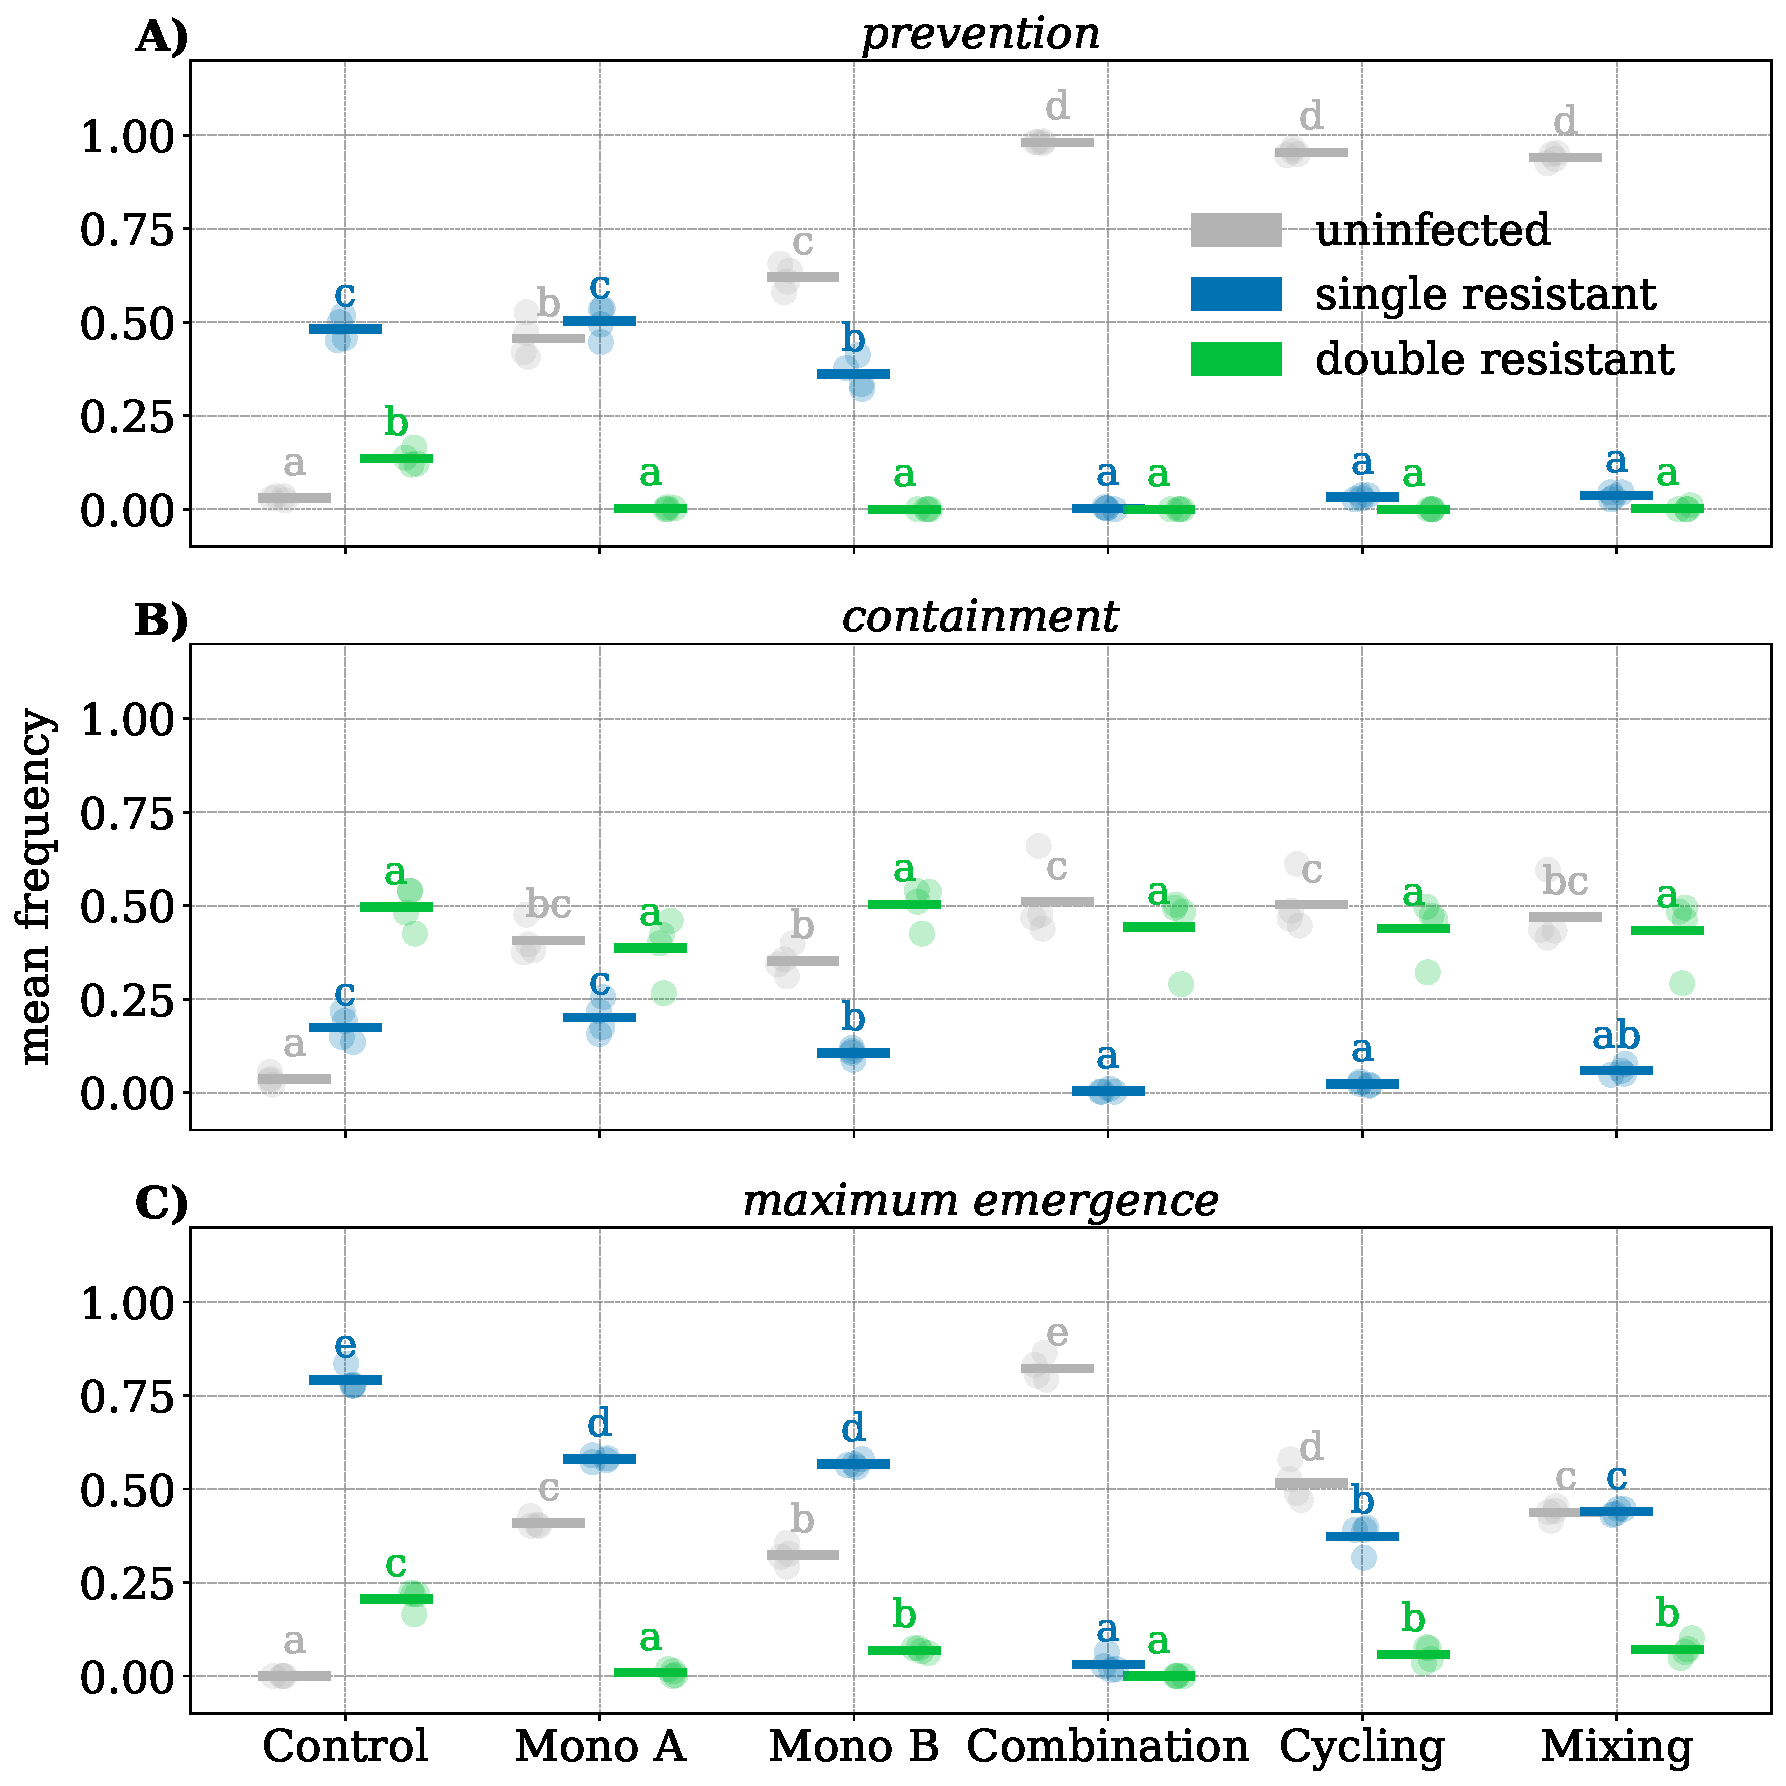
\includegraphics[width=\linewidth]{main_1/end_anova.pdf}
  \captionsetup{skip=2pt}
  \caption{
    Panels A--C show the mean frequency of uninfected (grey), single-resistant infected (blue), and double-resistant infected wells (green) during the last four transfers of the three scenarios.
    Circles represent replicates (n = 4), and bars represent means.
    Within resistance categories, bars not sharing a letter are significantly different (pairwise Tukey post hoc test, $p<0.05$; ANOVA tables and all p-values can be found in \sitab{34} -- \siref{50}).
  }
  \label{fig:end_anova}
\end{figure}

\paragraph{Multidrug strategies keep the overall number of infections lowest and best suppress single resistance.}
The \textit{prevention}~scenario is characterised by a moderate proportion of single-resistant admissions to the hospital ward, the absence of pre-existing double resistance, and a moderately spreading infection dynamic ($R_0 = 1.5$, \sieq{1},  \sisec{SI Methods}).
In this scenario, there are no differences between combination, mixing, and cycling on the frequency of uninfected, single-resistant-infected and double-resistant-infected wells (\panelref{fig:end_anova}{A}, time series in \sifig{2}).

However, all multidrug strategies are significantly better at suppressing single resistance and increasing the number of cleared wells than the single-drug strategies and the control without treatment (\panelref{fig:end_anova}{A}).
In all scenarios, combination therapy was one of the most successful treatment strategies in minimising single-resistant and overall infections.
At the same time, we observed most single and double resistance in the untreated control.
All strategies (but not the control) were able to clear sensitive infections effectively with clearance probabilities of 97\% for drug A, 73\% for drug B, and 86\% for AB (\sitab{8}).

\begin{figure}
  \centering
  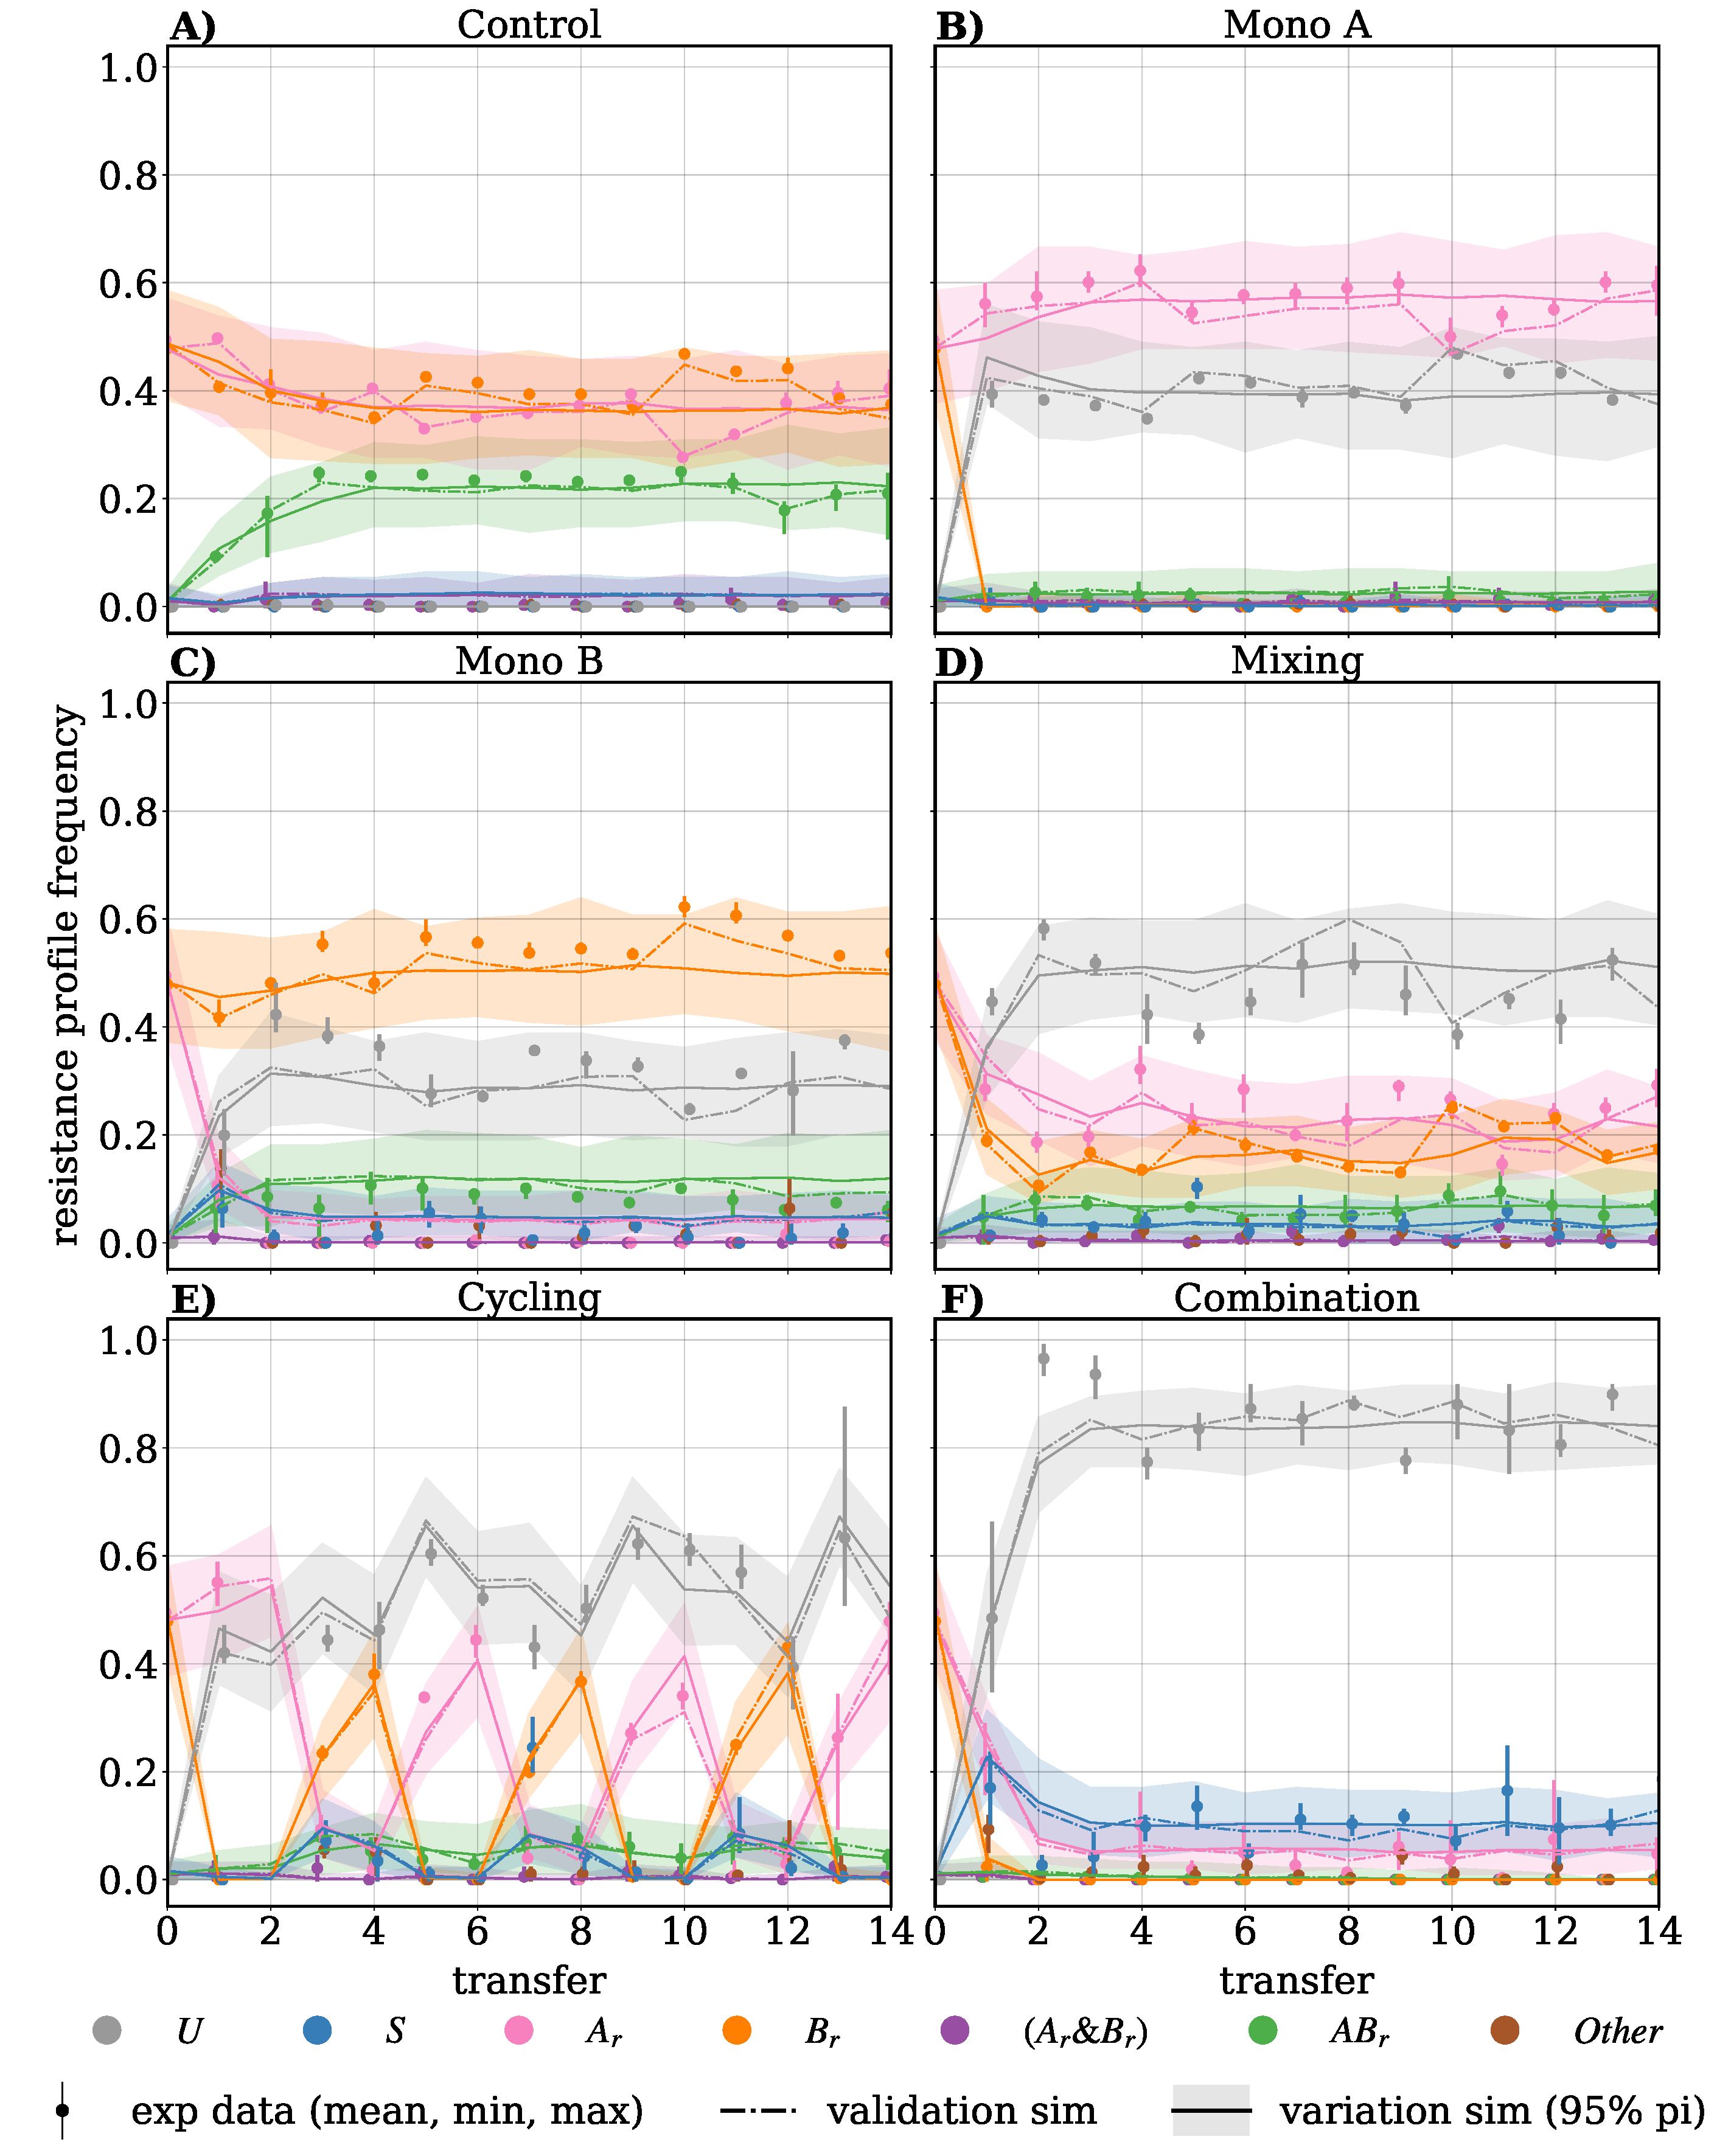
\includegraphics[width=\linewidth]{main_1/scen3_paper.pdf}
  \captionsetup{skip=2pt}
  \caption{
    Frequencies of resistance profiles over time during the \textit{maximum-emergence}~scenario. Panels (A--F) show the six tested strategies.
    Dots and bars show the mean and min/max interval of the four replicates.
    The dash-dotted line shows the mean value of 100 stochastic simulations based on the instruction set used in the \textit{in vitro} experiment (\textit{validation simulation}).
    The solid line shows the mean value of 100 simulations with randomly created instruction sets based on the parameter set used in the experiment (\textit{variation simulations}).
  The shaded error band indicates the 95-percentile interval between the \textit{variation simulations}.}
  \label{fig:exp3}
\end{figure}

\paragraph{All treatment strategies fail to contain pre-existing double resistance.}
The \textit{containment}~scenario explores a situation in which patients infected with double-resistant bacteria are continuously admitted to the hospital.
No strategy was able to contain the spread of double resistance, resulting in increased frequencies of double resistance ($> 40\%$) in all treatment arms at the conclusion of the experiment (\panelref{fig:end_anova}{B}).

%% emergence of double resistance in scenario III
\paragraph{Treatment strategies affect the emergence of double resistance.}
In our experiments, double resistance primarily emerges in wells inoculated with both single-resistance plasmids via HGT, as the evolution of de novo resistance (e.g. by point mutations) to high drug concentrations ($>50 \times$MIC) is unlikely.
As the inoculum volumes for turnover, infection, and passage are identical in our experiments, we do not distinguish between wells containing A-resistance ($A_r$) infecting wells containing B-resistance ($B_r$) or vice versa and simply refer to these events as superinfections.

During the \textit{prevention} and \textit{containment} scenario, we could not identify differences in the strategies' abilities to suppress the emergence of double resistance.
We attribute this to a lack of statistical power because we observed only a few instances of double resistance emerging, mostly in the untreated control.
To address this, we selected parameters for the \textit{maximum-emergence}~scenario designed to maximise superinfection opportunities between wells carrying complementary resistance.
To this end, all admitted patients carried bacteria with only one of the two resistance plasmids (at equal proportions).
In addition, we set the probability of admission and discharge to $\tau = 0.5$ and the infection probability to $\beta = 0.25$, resulting in a basic reproduction number $R_0 = 0.5$ (\sieq{1}).
An $R_0<1$ makes double resistance more likely to be replaced by newly admitted patients than to spread, thus maintaining a high potential for emergence.
We implement this scenario to explore emergence under a magnifying glass, being aware that it does not reflect a likely clinical situation. In this scenario, combination therapy and monotherapy with drug A lead to the lowest frequency of double resistance during the last four transfers (\panelref{fig:end_anova}{C}, \autoref{fig:exp3}).

For the \textit{maximum-emergence} scenario, we observed that combination therapy, cycling, and monotherapy with drug A were most effective in preventing newly emerging double resistance.
Combination was the only strategy in which we did not observe a single case of emerging double resistance after the first transfer (\panelref{fig:emergence}{A}).
Furthermore, combination therapy is the most successful treatment strategy in minimising the number of both single-resistant and overall infections, while the control leads to the highest number of double- and single-resistant, and overall infections.

\paragraph{Combination therapy suppresses the emergence of double resistance by preventing superinfections.}
Treatment strategies can impact the emergence of double resistance by suppressing superinfections.
The number of superinfections $n_{\mathcal S}$is dependent on the abundance of the single resistance carrying wells $A_r$ and $B_r$.
Hence, we expect the highest number of superinfections and most opportunities for emerging double resistance when both single resistances are unaffected by the treatment and the fewest if the treatment successfully suppresses both single resistances.
Our measurements confirmed these expectations during the \textit{maximum-emergence}~scenario.
Here $n_{\mathcal S}$is highest in the control group (no treatment) and lowest under combination therapy (\panelref{fig:emergence}{B}).

\paragraph{Treatment strategies influence the emergence of double resistance within superinfected wells.}
We observed the highest average frequency of superinfections developing double resistance $(\frac{n_{\mathcal E}}{n_{\mathcal S}})$ in antibiotic-free medium and in medium treated with antibiotic B (tetracycline).
In contrast, superinfections resulting in double resistance rarely occur in medium treated with antibiotic A (ceftazidime) or both drugs (\panelref{fig:emergence}{C}).
We think the impact of treatment on cell densities within superinfected wells (both in infected and infecting wells) can best explain these findings.

Firstly, applying a drug affects the in-well population dynamics of superinfected wells.
Reducing the cell density for one or both single-resistant strains within a superinfected well reduces the probability of bacteria with complementary resistance to encounter and conjugate (see \sisec{SI Results}).
As drug A (bactericidal) decreases the cell density faster than drug B (bacteriostatic), more conjugation opportunities occur in wells treated with drug B.

Secondly, the treatment strategies influence the number of transferred single-resistant bacteria that inoculate superinfections by curbing the bacterial density within the infecting wells (see \sisec{SI Results}).

Due to the differences in the abilities of drugs A and B to prevent conjugation, there are times (cycles) and places (beds) during cycling and mixing where using drug B offers increased opportunities for the emergence of double resistance, which is never the case with combination therapy.

\begin{figure}[t]
  \centering
  \setlength{\tabcolsep}{1em}
  \renewcommand{\arraystretch}{0}

  \begin{tabular}{@{}c c@{}}
    \begin{minipage}{0.6\textwidth}
      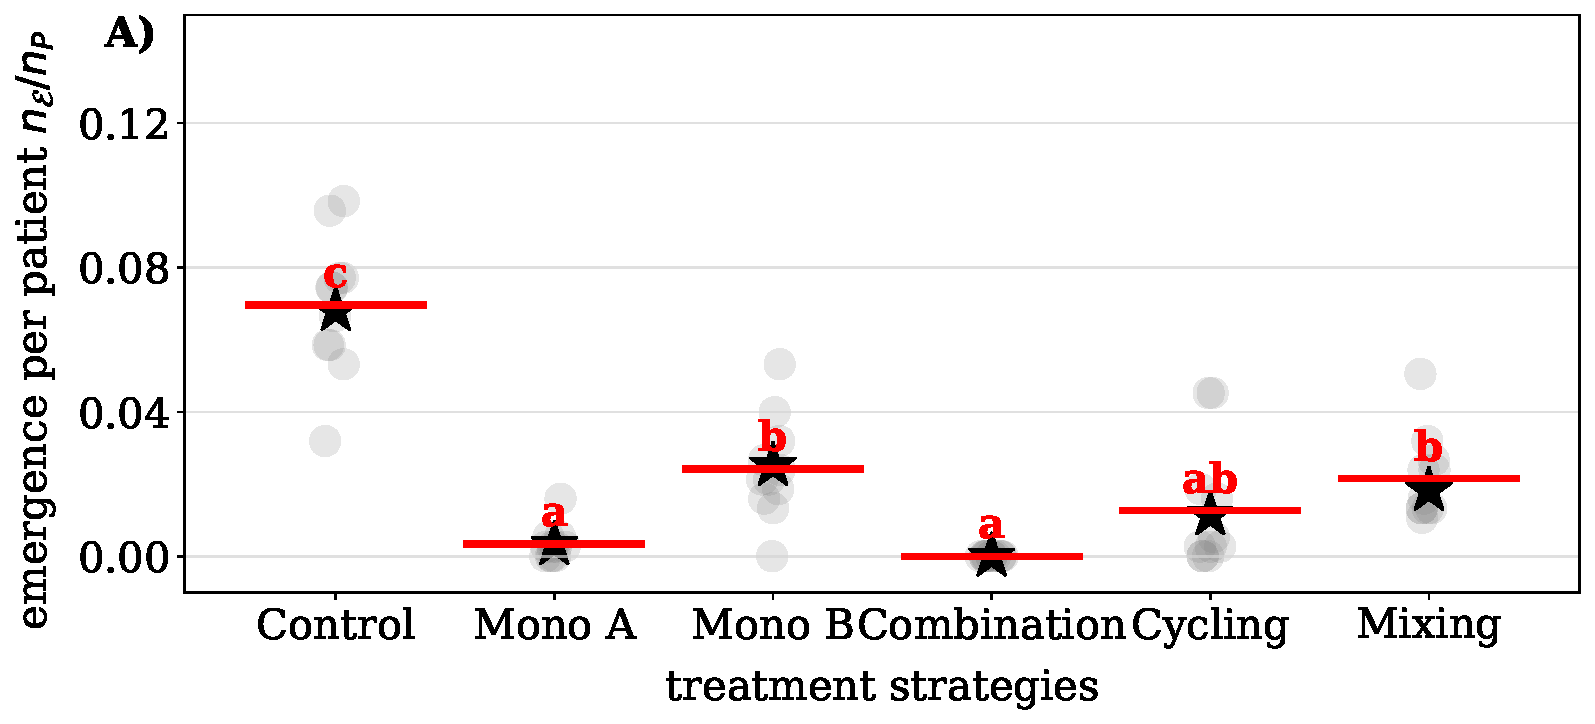
\includegraphics[height=4cm]{main_1/20220412_f_emergence_anova.pdf}
      \vspace{4pt}
      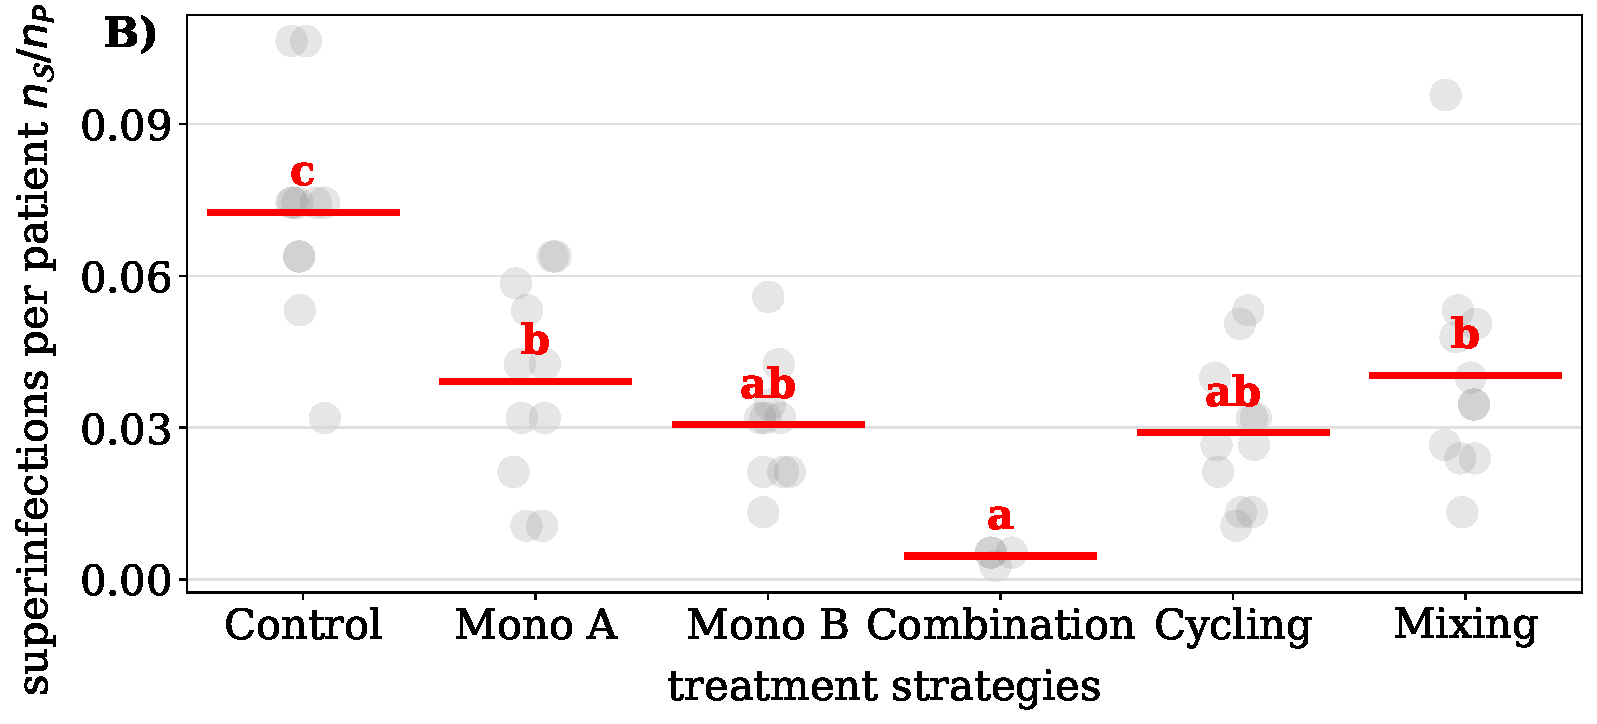
\includegraphics[height=4cm]{main_1/20220412_encounter_frequencies.pdf}
      \vspace{4pt}
      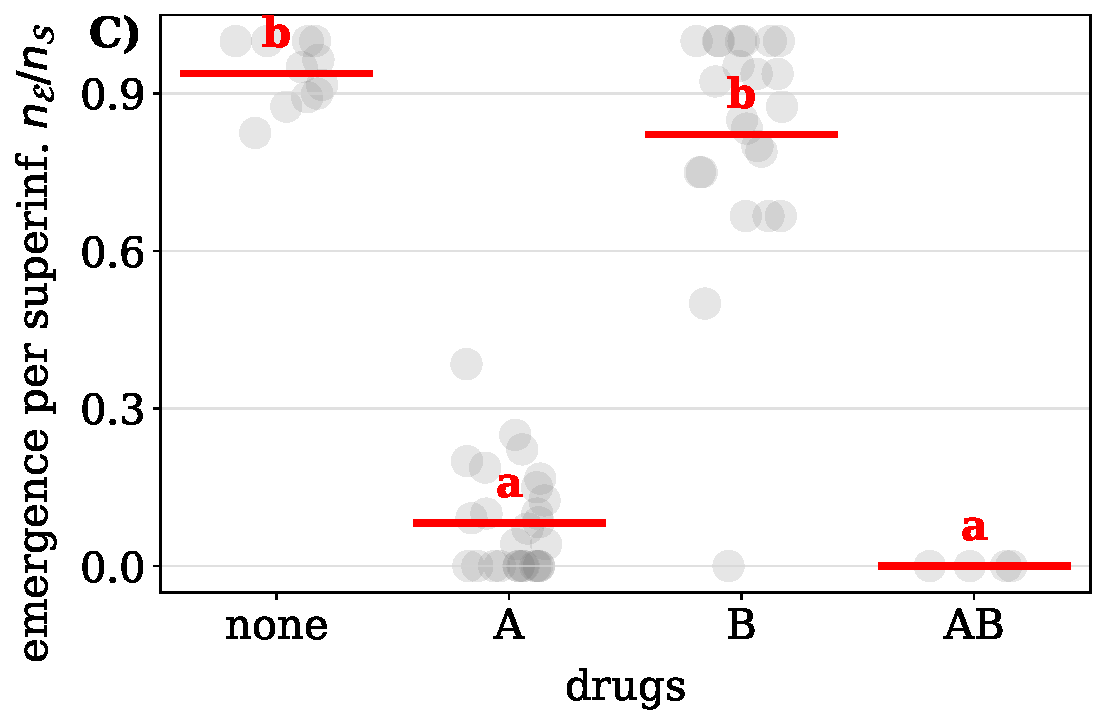
\includegraphics[height=4cm]{main_1/20220412_conjugation_prop.pdf}
    \end{minipage}
    &
    \begin{minipage}{0.39\textwidth}
      \captionsetup{skip=2pt}
      \caption{
        Analysis of the emergence of double resistance \textit{in vitro} and superinfection between single resistant $A_r$ and $B_r$ wells during the \textit{maximum-emergence}~scenario, from transfer four onwards.
        Each dot corresponds to data from a single plate, with each plate representing a distinct treatment arm, encompassing 376 patients for one transfer.
        Mean values are represented by red bars.
        Bars not sharing a letter are significantly different ($p < 0.05$, ANOVA tables and pairwise Tukey post hoc results can be found in \sitab{51} -- \siref{56}).
      \textbf{A)} Number of newly emerged cases of double resistance per plate ($n_{{\mathcal E}}$), normalised to the total number of patients ($n_P = 376$).
    \textbf{B)} Number of superinfections per plate ($n_{\mathcal S}$), normalised to $n_P$.
  \textbf{C)} Proportion of superinfected wells treated with A, B, AB, or none that develop double resistance.
}
\label{fig:emergence}
\end{minipage}
\end{tabular}
\end{figure}

\paragraph{Computational model corroborates the robustness of experimental outcomes.}
The experiments are conducted by a liquid handling platform that carries out predefined instructions, specifying which infections occur and who is admitted or discharged.
The instructions are randomized based on parameter sets we defined for each scenario, including the overall infection and turnover probability as well as the distribution of the resistance profiles of admitted patients.
We call the entirety of all instructions that come up during one experiment an `instruction set'.
Due to the scale and technical complexity of the experiments, it was not feasible to carry out individual instruction sets for each replicate, so we opted to apply the same instruction sets for all replicates.
This raises the question of whether the experimental results are a consequence of a specific instance of this random process and whether they are robust to the randomisation in the instruction set.
To address this, we developed a discrete-time stochastic model comprising 94 individual \textit{in silico} patients mimicking the epidemiological dynamics of the experiment (\sisec{SI Computational Model}).
The model was parametrised, but not fitted, with transition probabilities (\sitab{18}--\siref{25}) that we estimated based on the transition frequencies measured \textit{in vitro}.
We used the same transition probabilities in the simulations for all scenarios.

First, we validated the model by averaging 100 \textit{validation simulations}, each employing the identical instruction sets used \textit{in vitro}.
The aim of the \textit{validation simulations} is to recreate the experiments \textit{in silico} (\sifig{3B}).
We found that the simulation results are in good agreement with the experimental data, indicating that the model reflects the dynamics observed in the \textit{in vitro} experiments well (see \autoref{fig:exp3}, \sifig{2}, and \sifig{4}).
One exception is the spread of A-resistance during the \textit{prevention}~scenario in control and Mono~A.
This could indicate an increased number of contaminations at the beginning of the \textit{prevention}~scenario.
We also observe some discrepancies for the spread of double resistance during the \textit{prevention}~scenario, which we attribute to contamination artefacts in the transition probabilities (see \sisec{SI Computational Model}).

Second, we averaged 100 \textit{variation simulations} to assess the robustness of the experimental outcomes against variations in the instruction sets.
In these \textit{variation simulations}, each of the 100 instruction sets was randomized based on the same three parameter sets used \textit{in vitro} (\sifig{3C}).
Differences between the \textit{validation} and \textit{variation simulations} indicate differences in outcome due to the randomization of the instruction sets.
For instance, with a turnover probability $\tau = 0.2$ and an admission probability $c_A = 0.05$, we expect $0.94$ $A_r$ admissions per transfer. However, random fluctuations can result in either more (or fewer) $A_r$ admissions, leading to a temporarily higher (or lower) frequency of $A_r$ in the \textit{validation simulations}, creating a temporary spread between the \textit{validation} and \textit{variation simulations}.
We observed that the \textit{validation simulations} fluctuate around the \textit{variation simulations} and never diverge far (see \autoref{fig:exp3}, \sifig{2}, and \sifig{4}), indicating robustness of the experimental results to the randomisation of the instruction sets.

\paragraph{\textit{In silico} sensitivity analysis indicates that the superiority of combination therapy is robust.}
Given that the \textit{validation simulations} agreed well with the experiments, we used the model to perform an \textit{in silico} parameter sensitivity analysis of the experimental results (\sifig{3D}).
To this end, we ran ten simulations for each of 20,000 randomly generated parameter sets by varying the turnover and infection probability and the five sampling proportions for incoming patients: ($\tau$, $\beta$, $c_S$, $c_{A_r}$, $c_{B_r}$, $c_{AB_r}$, $c_U$).
For half of the parameter sets, we forced the frequency of incoming patients with double resistance ($c_{AB_r}$) to zero.

We used the frequency of uninfected \textit{in silico} patients to measure treatment success.
Using this criterion, the control strategy (no treatment) always performed worst, and accordingly, we excluded this treatment arm from the following analysis.
Strategies were then classified as (i) 'single winners' if they are significantly better than all other strategies; (ii) 'winners' if they are not outperformed by any other strategy; (iii) 'losers' if they do not outperform at least one other strategy; or (iv) 'single losers' if all other strategies outperform them.

In parameter sets with and without pre-existing double resistance, combination therapy ranks most often as one of the best strategies (87\%  and 98\%, respectively).
It is the single best strategy in 55\% of the tested parameter sets with pre-existing double resistance and in 93\% of cases without pre-existing double resistance (\autoref{fig:senstivity_analysis}, \sitab{14},~\sitab{15}).

In some situations (for example, when one strategy is much worse than all others), it is more important to avoid the worst strategy than selecting the very best strategy among the good ones.
Our analysis finds that combination therapy is almost never among the worst strategies, while usually one of the two monotherapies performs worst.
As expected, single-drug strategies perform particularly poorly when there is a high frequency of pre-existing single-resistance to the applied drug (\sitab{11}, \sitab{13}).

Cycling and mixing lose substantially less than the monotherapies but are rarely the single best strategy.

\begin{figure}[h]
\centering
\setlength{\tabcolsep}{1em}
\renewcommand{\arraystretch}{0}

\begin{tabular}{@{}c c@{}}
\begin{minipage}{0.69\textwidth}
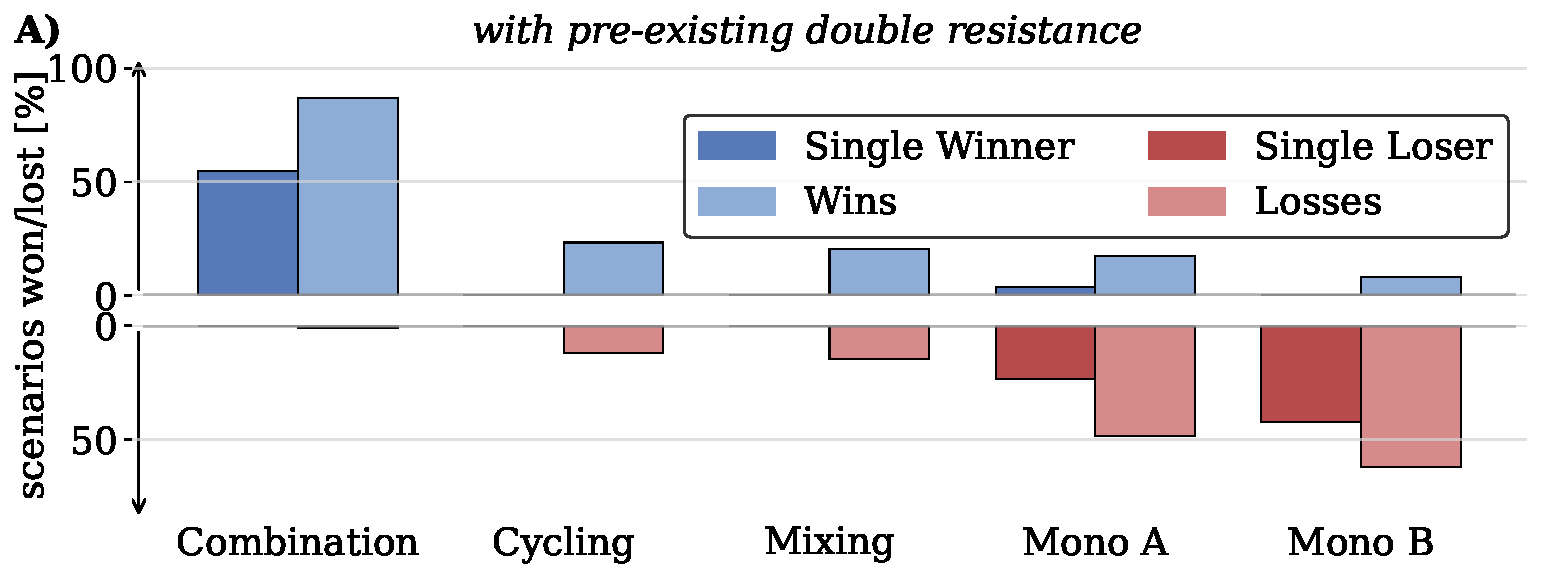
\includegraphics[width=\textwidth]{main_1/wins_and_losses_preexisting.pdf}
\vspace{4pt}
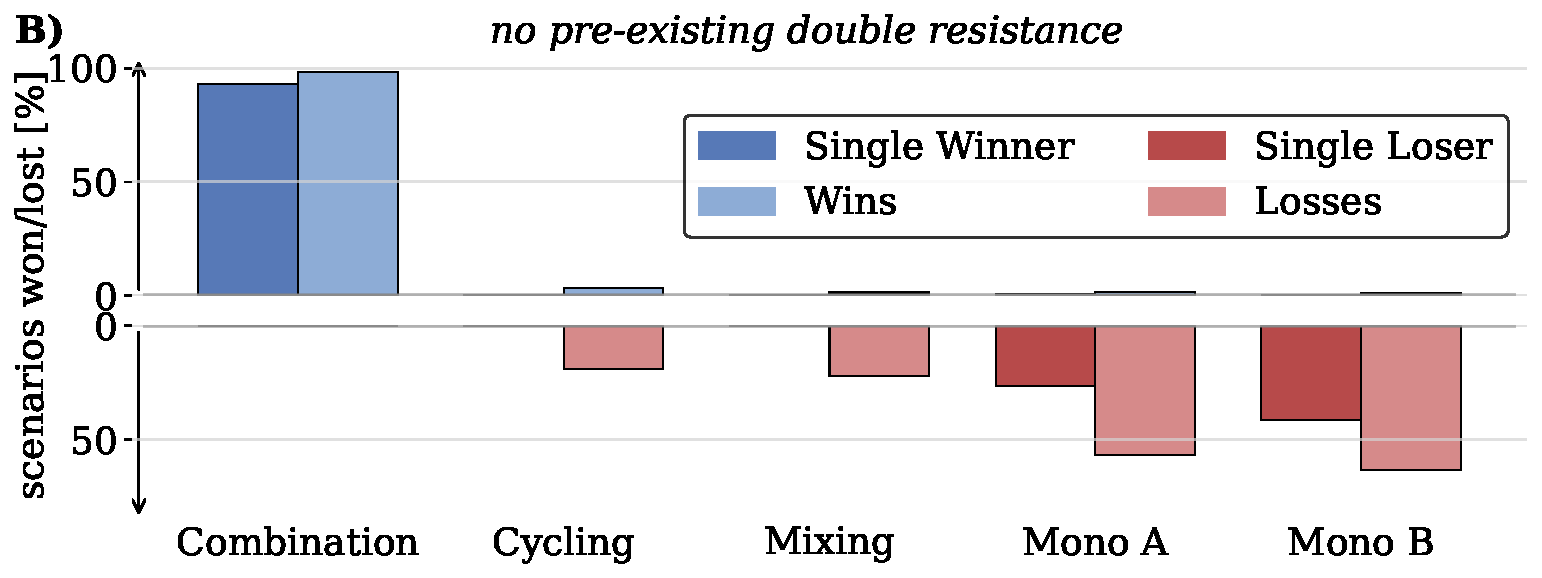
\includegraphics[width=\textwidth]{main_1/wins_and_losses_no_preex.pdf}
\end{minipage}
&
\begin{minipage}{0.3\textwidth}
\captionsetup{skip=2pt}
\caption{
  Effectiveness of the five treatment strategies in maximising the frequency of uninfected individuals across randomly generated parameter sets.
  Strategies not significantly better than any other are marked as losers (pastel red), and those significantly worse than all others as single losers (dark red).
  Strategies not significantly worse than any other are classified as winners (pastel blue), and those significantly better than all others as single winners (dark blue).
  Strategies without significant differences were excluded.
  \textbf{(A)} 10{,}000 parameter sets with pre-existing double resistance. 606/10{,}000 sets yielded no significant difference between the strategies.
  \textbf{(B)} 10{,}000 parameter sets without pre-existing double resistance. 100/10{,}000 sets yielded no significant difference between the strategies.
}
\label{fig:senstivity_analysis}
\end{minipage}
\end{tabular}
\end{figure}
